\chapter{Specific Requirements} \label{chap3}

\section{Functional Requirements}
Functional requirements should define the fundamental actions that must take place in the software in accepting and processing the inputs and in processing and generating the outputs.

\begin{itemize}
	\item [\textbf{G01}] $\rightarrow$ To allow a visitor to sign up, the system shall provide functionalities to:
	\begin{itemize}
		\item [\textbf{R01}] Check the validity and correctness of the information provided by the visitor (personal information, password, payment information)
		\item [\textbf{R02}] Check if the user is already registered into the system 
	\end{itemize}
	
	\item [\textbf{G02}] $\rightarrow$ To allow a visitor to login, the system shall provide functionalities to:
	\begin{itemize}
		\item [\textbf{R03}] Check if username and password provided by the visitor correspond to an existing user, authorized to use the system
		\item [\textbf{R04}] Prevent unauthorized or banned users from accessing the system 
	\end{itemize}
	
	\item [\textbf{G03}] \& [\textbf{G04}] $\rightarrow$ To allow a passenger to request and to reserve a taxi, the system shall provide functionalities to:
	\begin{itemize}
		\item [\textbf{R05}] Obtain the passenger location
		\item [\textbf{R06}] Access the queue associated to the right taxi zone
		\item [\textbf{R07}] Check the availability of the taxi drivers
		\item [\textbf{R08}] Iteratively contact all the taxi drivers of the queue starting from the first one until one of them accepts the call
		\item [\textbf{R09}] Iteratively search for an available taxi driver inside adjacent zones in the case that the right zone has an empty queue or all the contacted taxi drivers had declined the request
	\end{itemize}
	
	\item [\textbf{G05}] $\rightarrow$ To allow a passenger to receive information about the incoming taxi the system shall provide functionalities to:
	\begin{itemize}
		\item [\textbf{R10}] Obtain the taxi driver position and the passenger position and estimate the time needed by the taxi driver to reach the passenger
		\item [\textbf{R11}] Obtain the taxicab unique identifier from the taxi drivers database
	\end{itemize}
	
	\item [\textbf{G06}] $\rightarrow$ To allow a passenger to share a ride, the system shall provide functionalities to:
	\begin{itemize}
		\item [\textbf{R12}] Check for each request or reservation if the passenger had selected the sharing function
		\item [\textbf{R13}] Compare routes that start from the same taxi zone and determine whether or not they can be merged into one, according to specific rules of comparison
		\item [\textbf{R14}] Calculate the correct distribution of the fee according to specific rules based on the percentage of the kilometers shared with others or traveled alone
		\item [\textbf{R15}] Elaborate an optimal route for taking every passenger to the right destination and show it to the taxi driver
	\end{itemize}

	\item [\textbf{G07}] $\rightarrow$ To allow a passenger to receive receipts after each completed ride, the system shall provide functionalities to:
	\begin{itemize}
		\item [\textbf{R16}] Keep track of the actual route followed by the taxi driver and keep track of the actual duration of the ride
	\end{itemize}
	
	\item [\textbf{G08}] \& [\textbf{G10}] $\rightarrow$ To allow a taxi driver to signal whether he is available or not, and to accept/decline an incoming request, the system shall provide functionalities to:
	\begin{itemize}
		\item [\textbf{R17}] Monitor and collect inputs from taxi drivers
	\end{itemize}
	
	\item [\textbf{G09}] $\rightarrow$ To allow a taxi driver to receive incoming requests, the system shall provide functionalities to:
	\begin{itemize}
		\item [\textbf{R18}] Contact taxi drivers and forward them all the information about the proposed request (position of the passenger, destination of the passenger, sharing option enabled or not)
	\end{itemize}		
	
	\item [\textbf{G11}] $\rightarrow$ To allow a taxi driver to visualize information about the optimal route for the ongoing ride, the system shall provide functionalities to:
	\begin{itemize}
		\item [\textbf{R19}] Retrieve the taxi location and the locations of all the passengers of the ride
		\item [\textbf{R20}] Access and query the map provider service to obtain an updated map with information about traffic, smashes, road construction sites
	\end{itemize}
	
	\item [\textbf{G12}] $\rightarrow$ To allow a developer to add new features, the system shall provide functionalities to:
	\begin{itemize}
		\item [\textbf{R21}] 
	\end{itemize}
\end{itemize}

\section{Non Functional Requirements}

\subsection{External Interfaces}
\textit{\textbf{Hardware Interface:}}\\
Device should be enabled with Internet and GPS receiver.\\
\textit{\textbf{Software interface:}}\\
The user's browser should be HTML5 compatible and the resolution should be at least 1280x720 for a satisfactory user experience.\\

\subsection{User Interfaces}
Here are presented some mockups that represent an idea of the structure of the application pages:

\subsubsection{Login}
The mockup in Figure \ref{fig:login} shows the Login Page of MyTaxiService. Here users can log in to the application.

\begin{figure}[htbp]
\centering
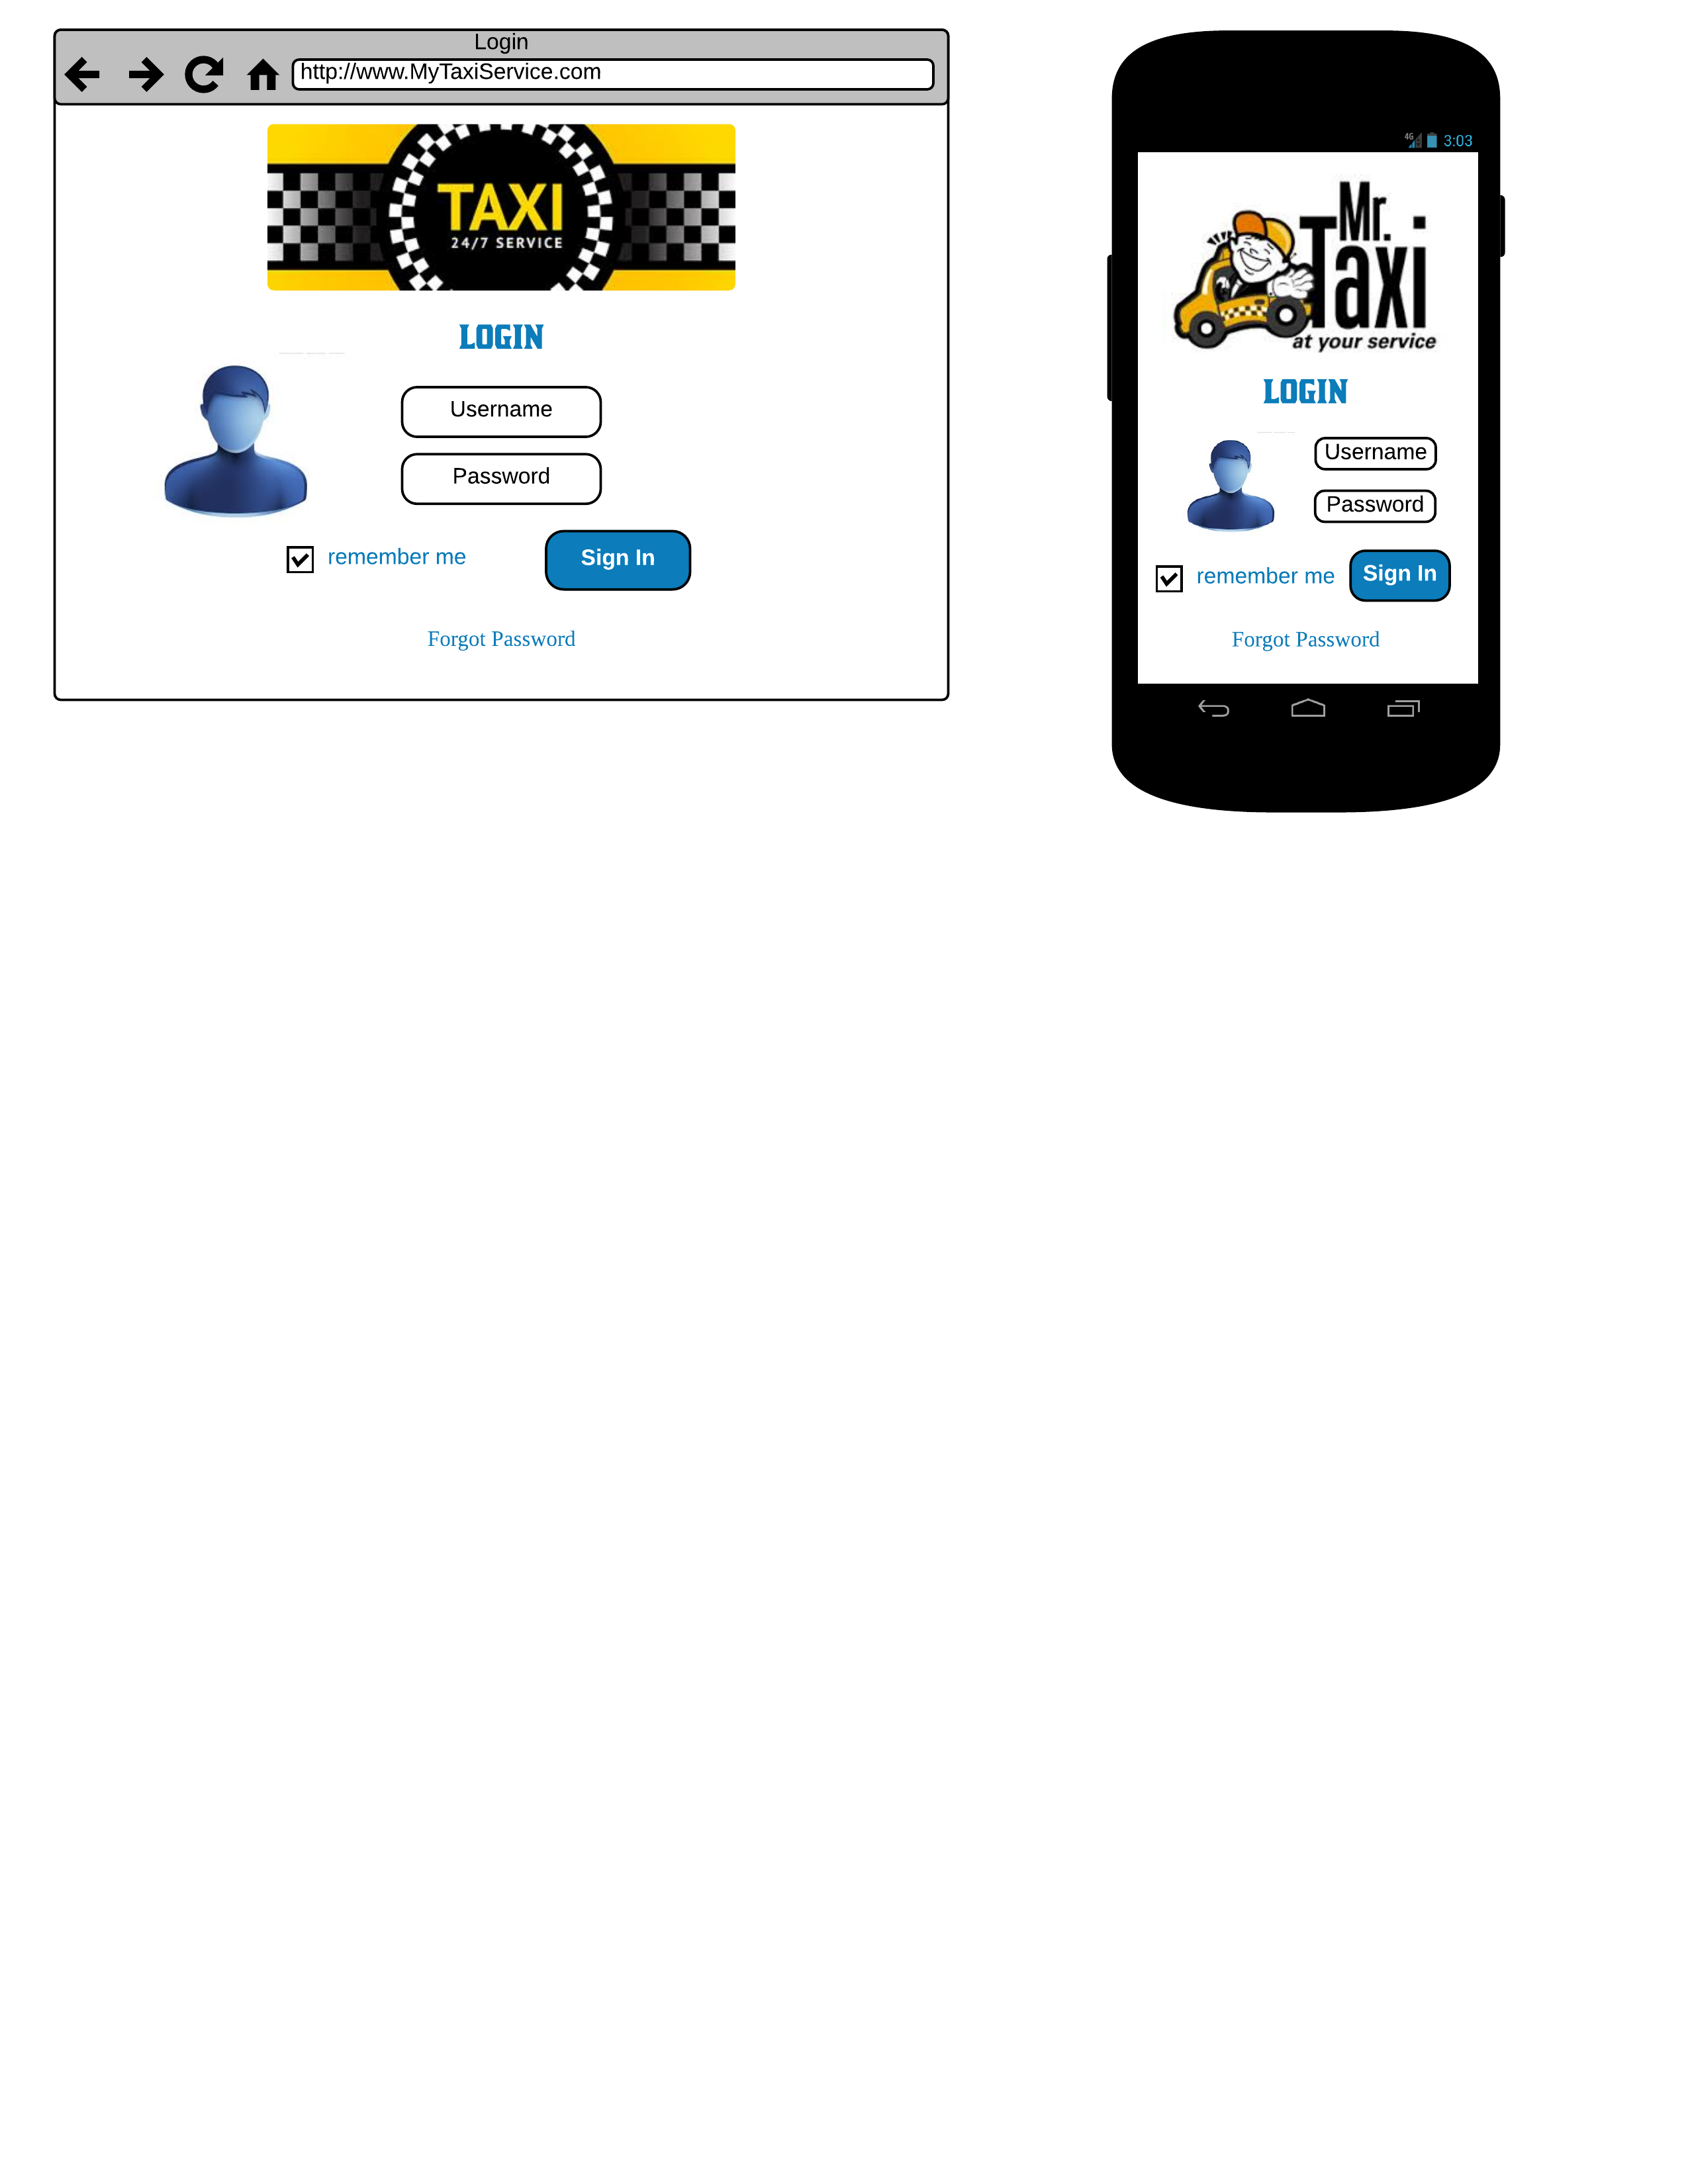
\includegraphics[width=\textwidth]{cpt/img/Login}
\caption{Login Page mockup}
\label{fig:login}
\end{figure}

\subsubsection{Registration Form}
The mockup in Figure \ref{fig:regform} shows the Registration Form Page that visitors can access.

\begin{figure}[htbp]
\centering
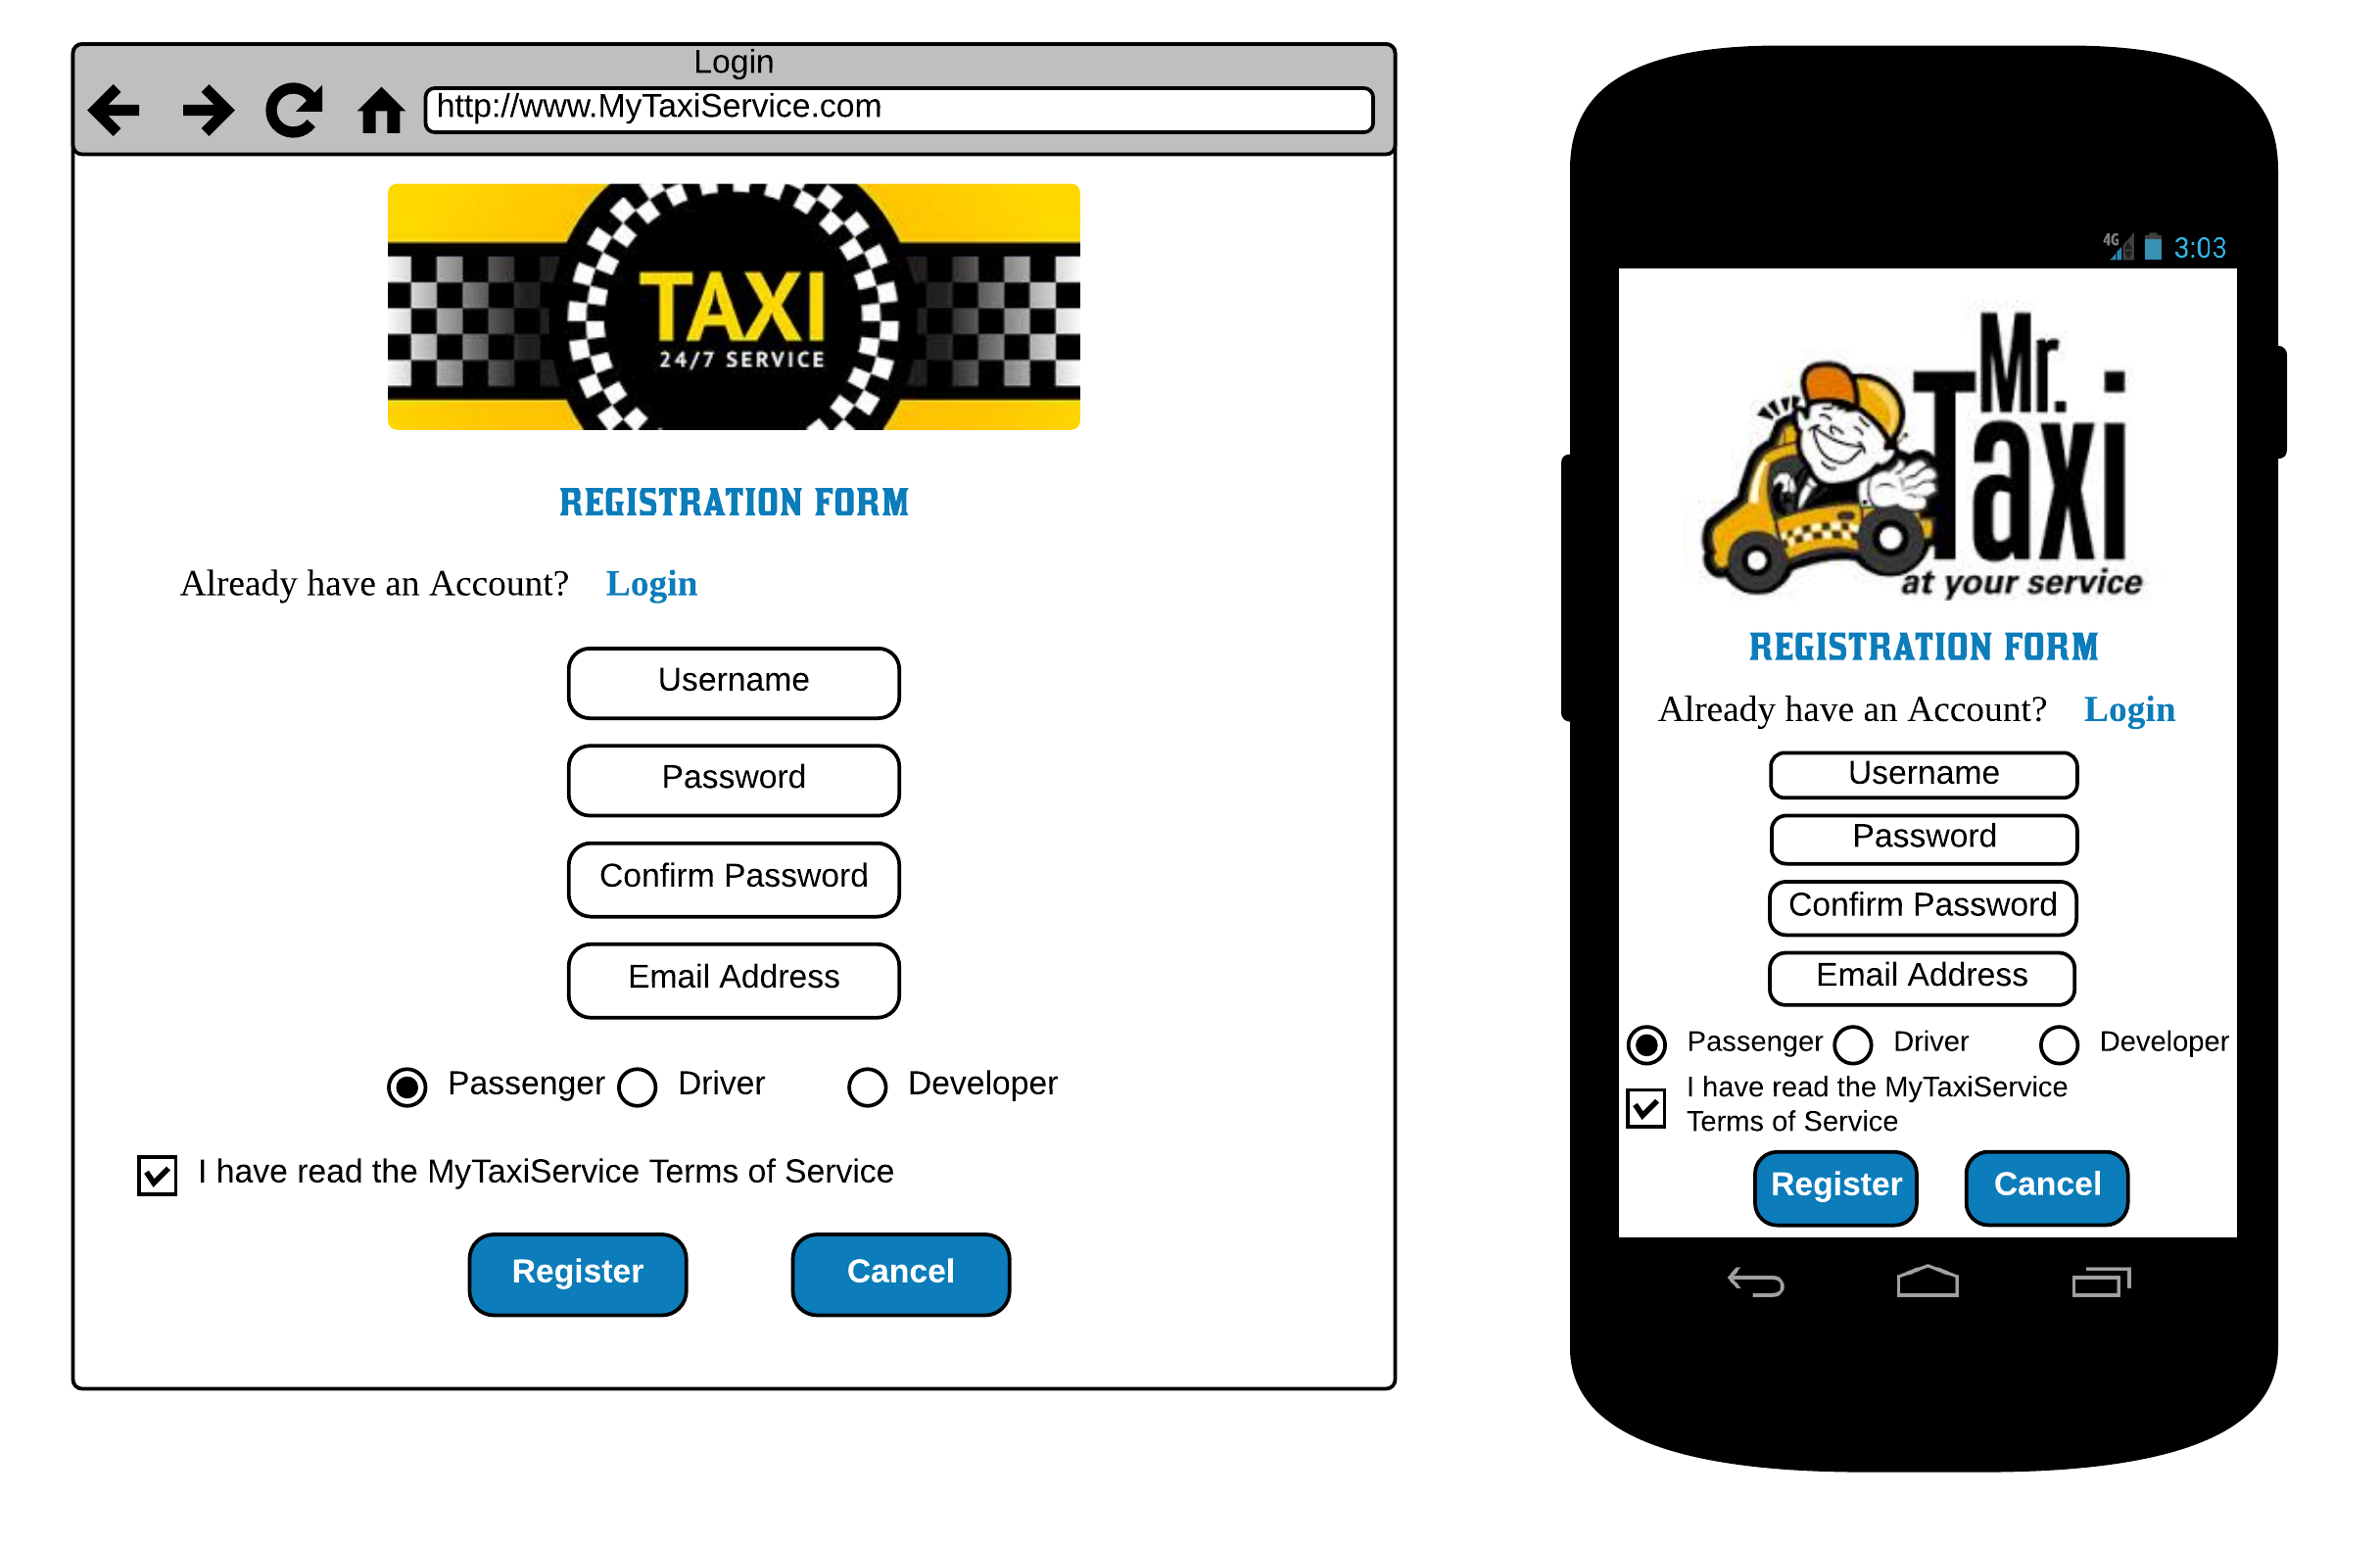
\includegraphics[width=\textwidth]{cpt/img/RegForm}
\caption{Registration Form mockup}
\label{fig:regform}
\end{figure}

\subsubsection{Passenger Home Page}
The mockup in Figure \ref{fig:passhome} shows the Home Page for a Passenger user.

\begin{figure}[htbp]
\centering
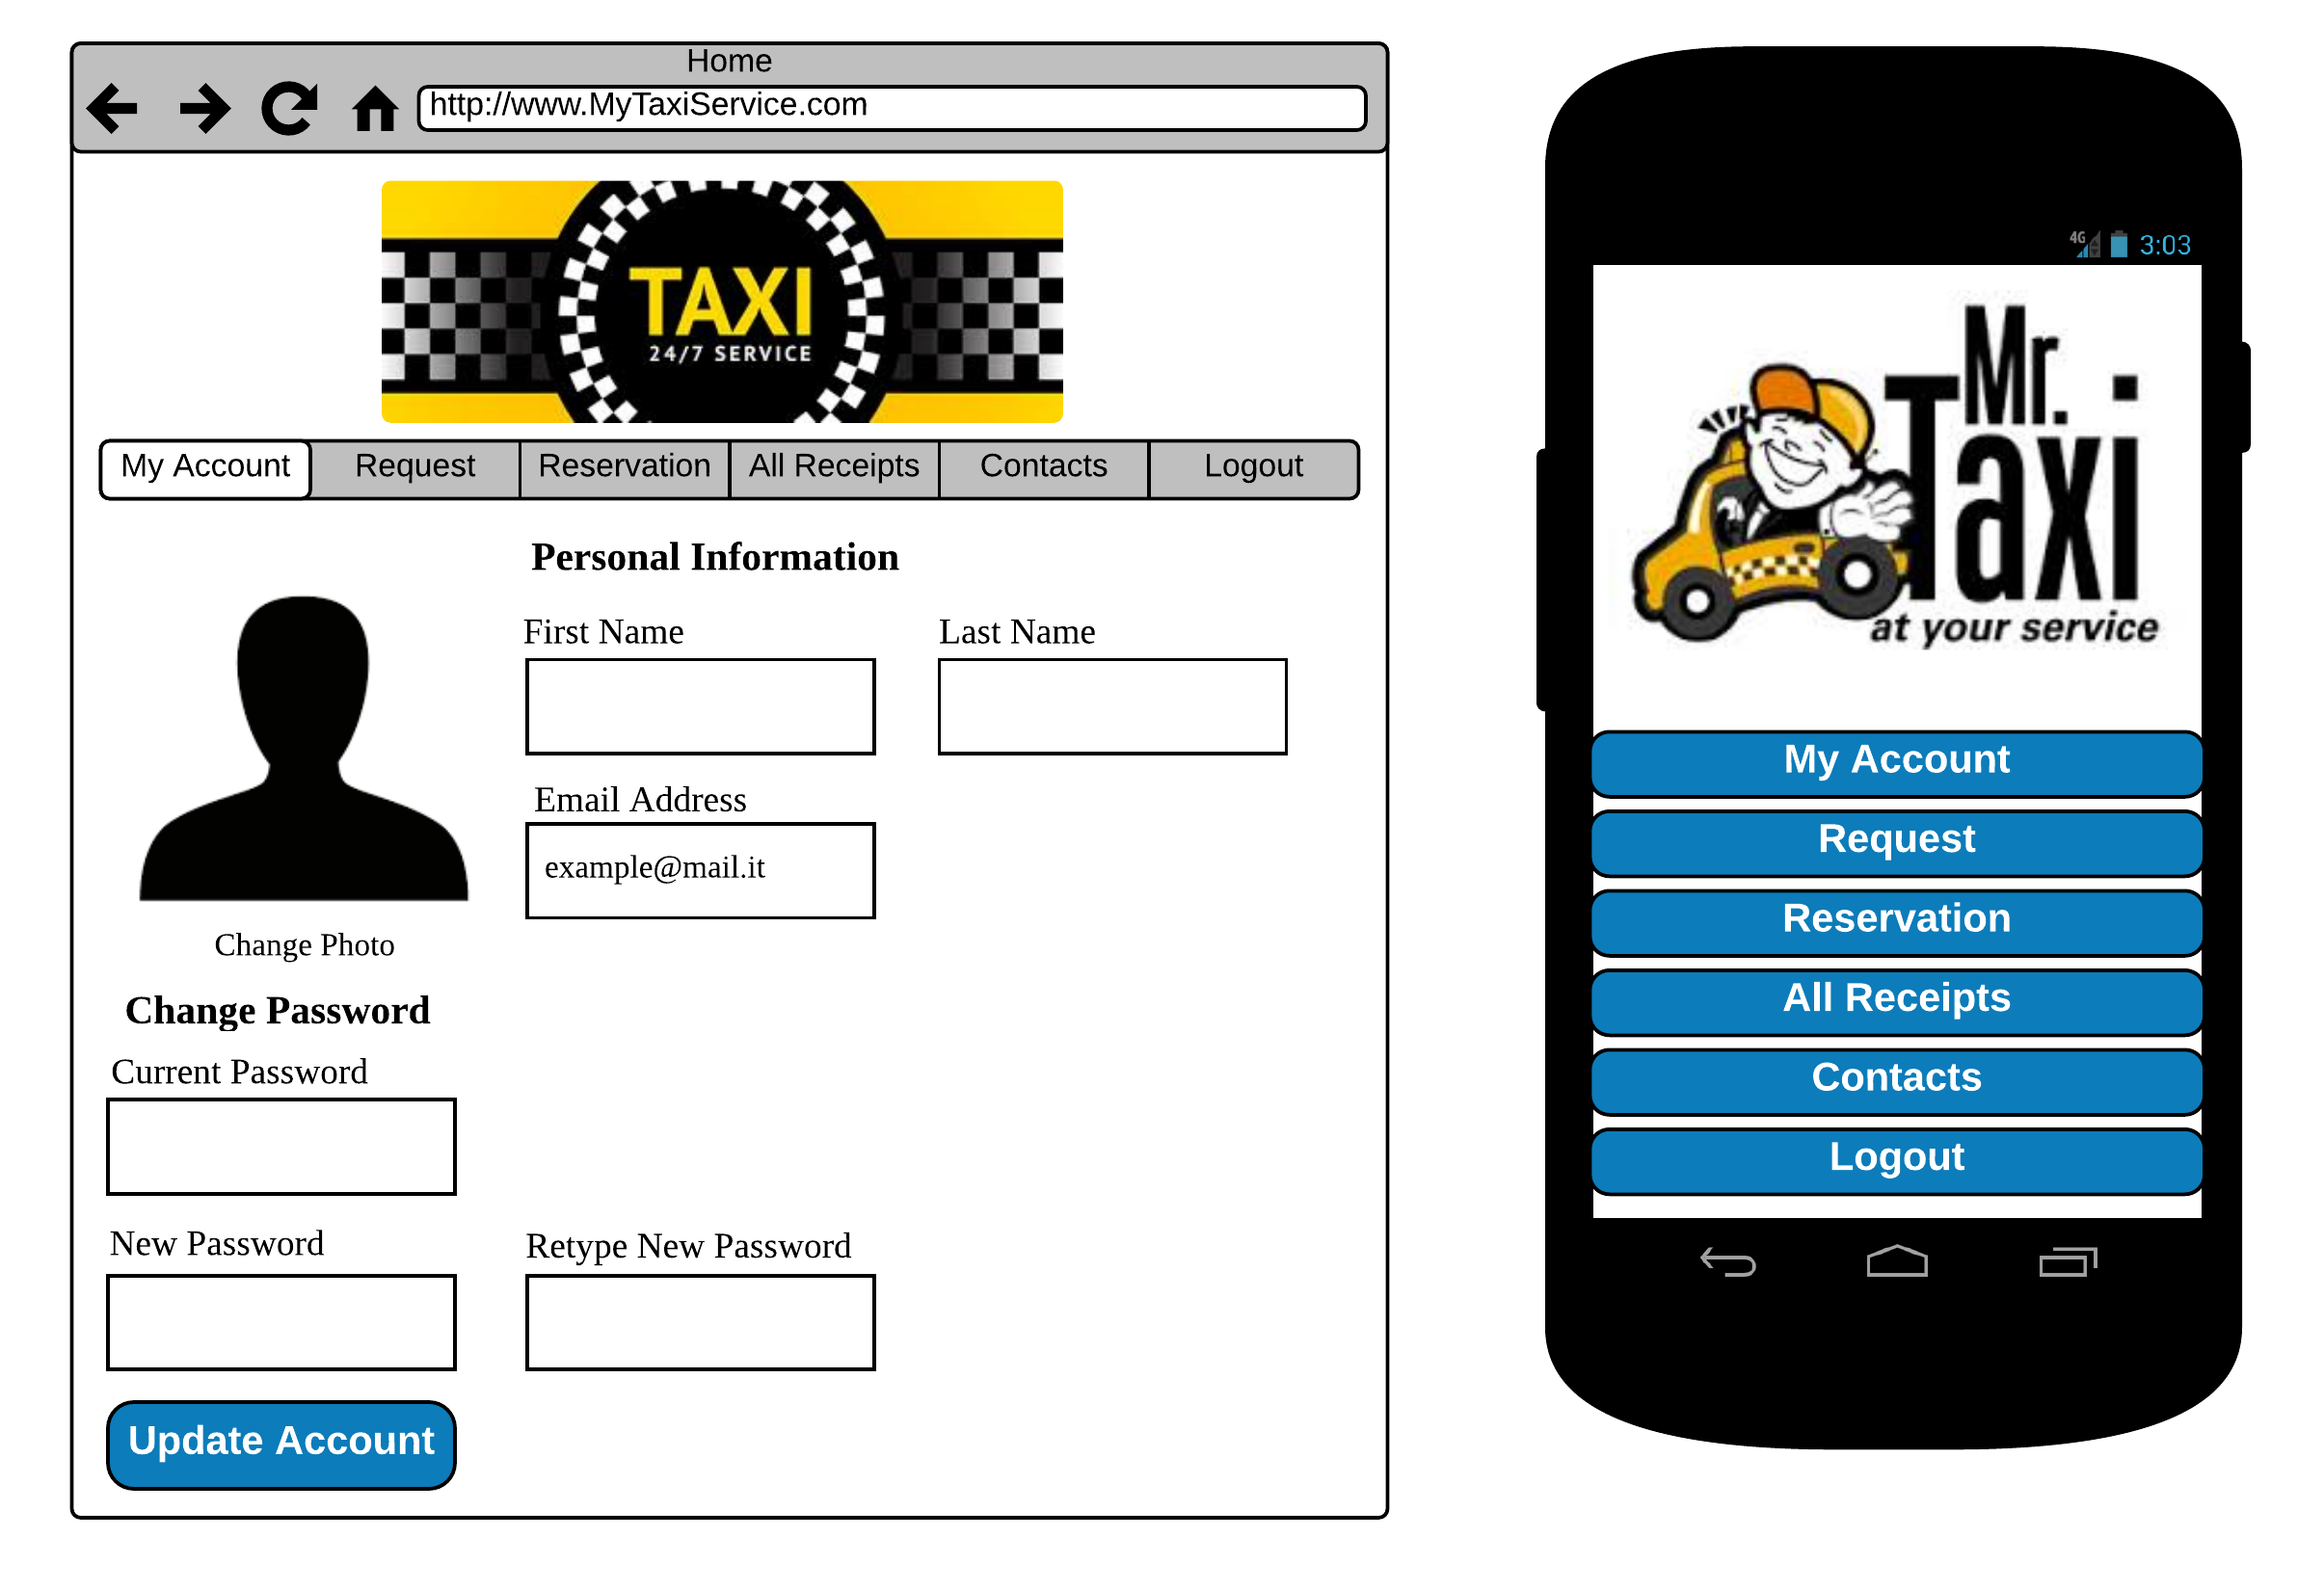
\includegraphics[width=\textwidth]{cpt/img/PassHome}
\caption{Passenger Home Page mockup}
\label{fig:passhome}
\end{figure}

\subsubsection{Passenger Request Page and Reservation Page}
The mockups in Figure \ref{fig:reqres} shows the Request and the Reservation Pages for a Passenger.

\begin{figure}[htbp]
\centering
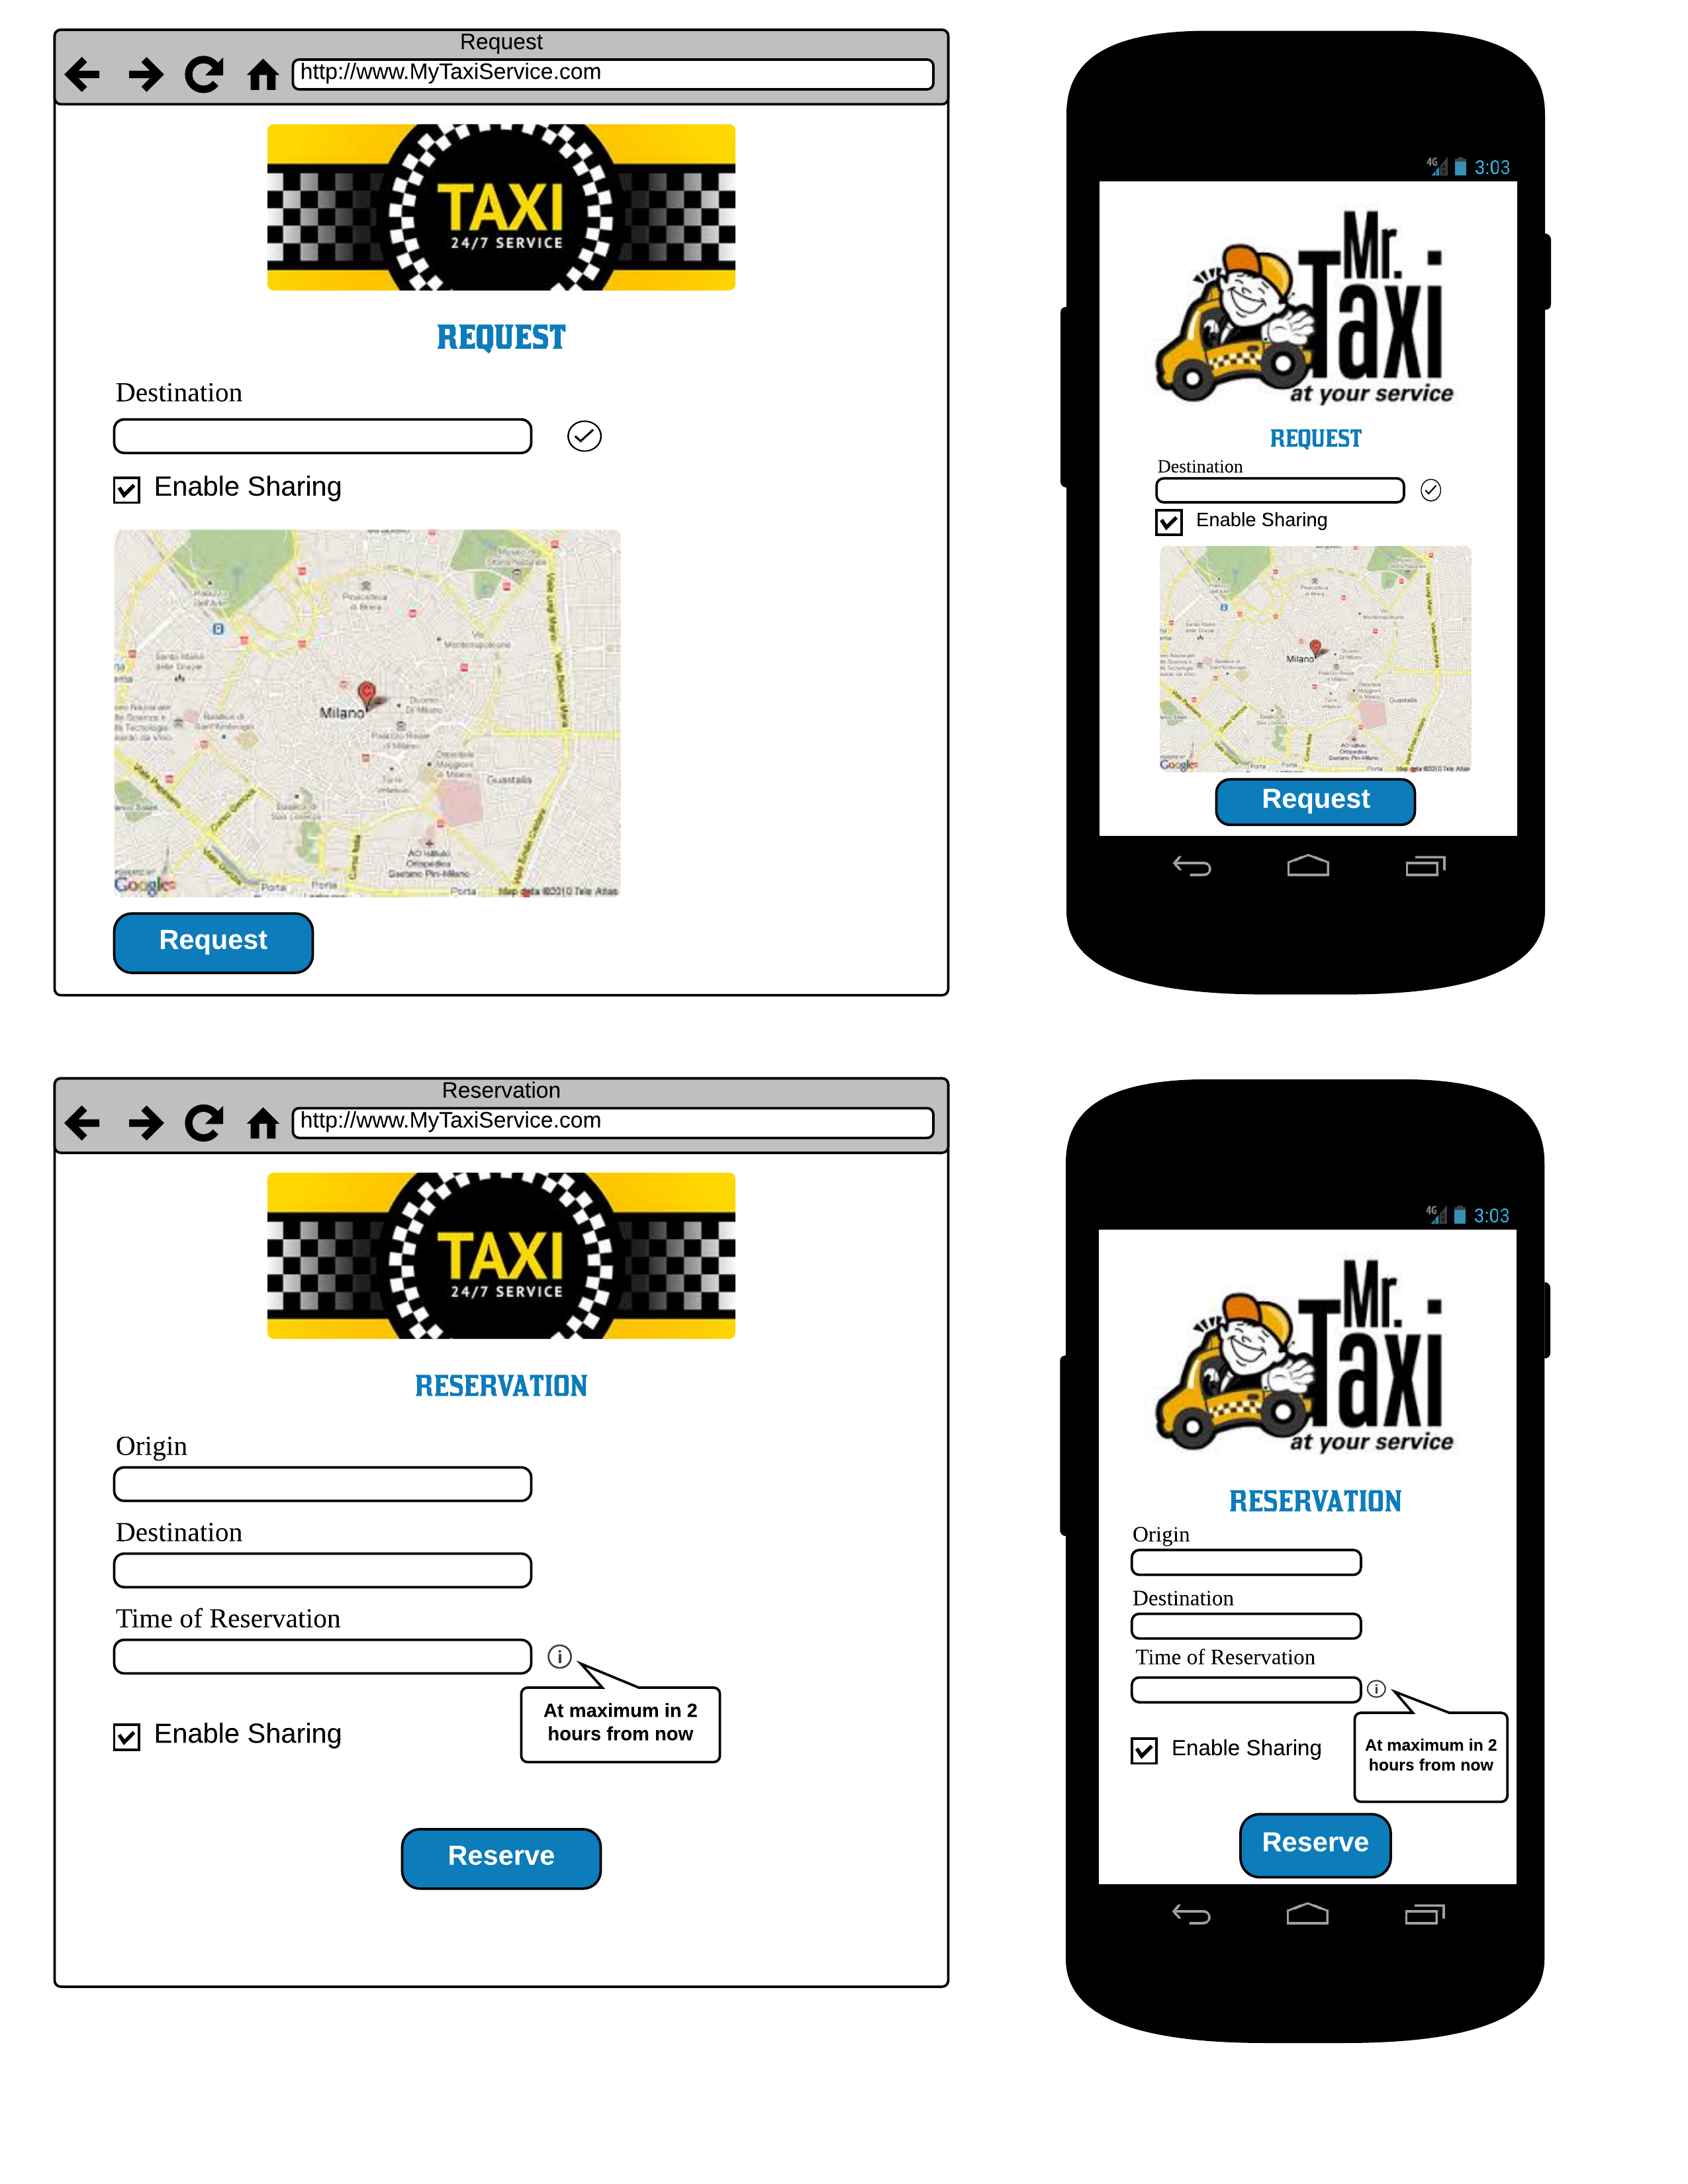
\includegraphics[width=\textwidth]{cpt/img/PassReqRes}
\caption{Passenger Request Page \& Reservation Page mockups}
\label{fig:reqres}
\end{figure}

\subsubsection{Taxi Driver Home Page}
The mockup in Figure \ref{fig:drivhome} shows the Home Page for a Taxi Driver user.

\begin{figure}[htbp]
\centering
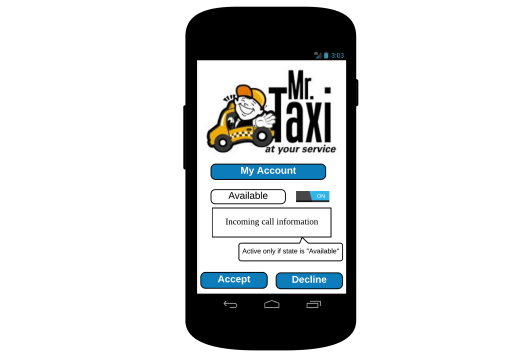
\includegraphics[width=\textwidth]{cpt/img/DriverHome}
\caption{Taxi Driver Home Page mockup}
\label{fig:drivhome}
\end{figure}

\subsubsection{Taxi Driver Accepted Call Page}
The mockup in Figure \ref{fig:accpage} shows the Page for a Taxi Driver user that accepts a call.

\begin{figure}[htbp]
\centering
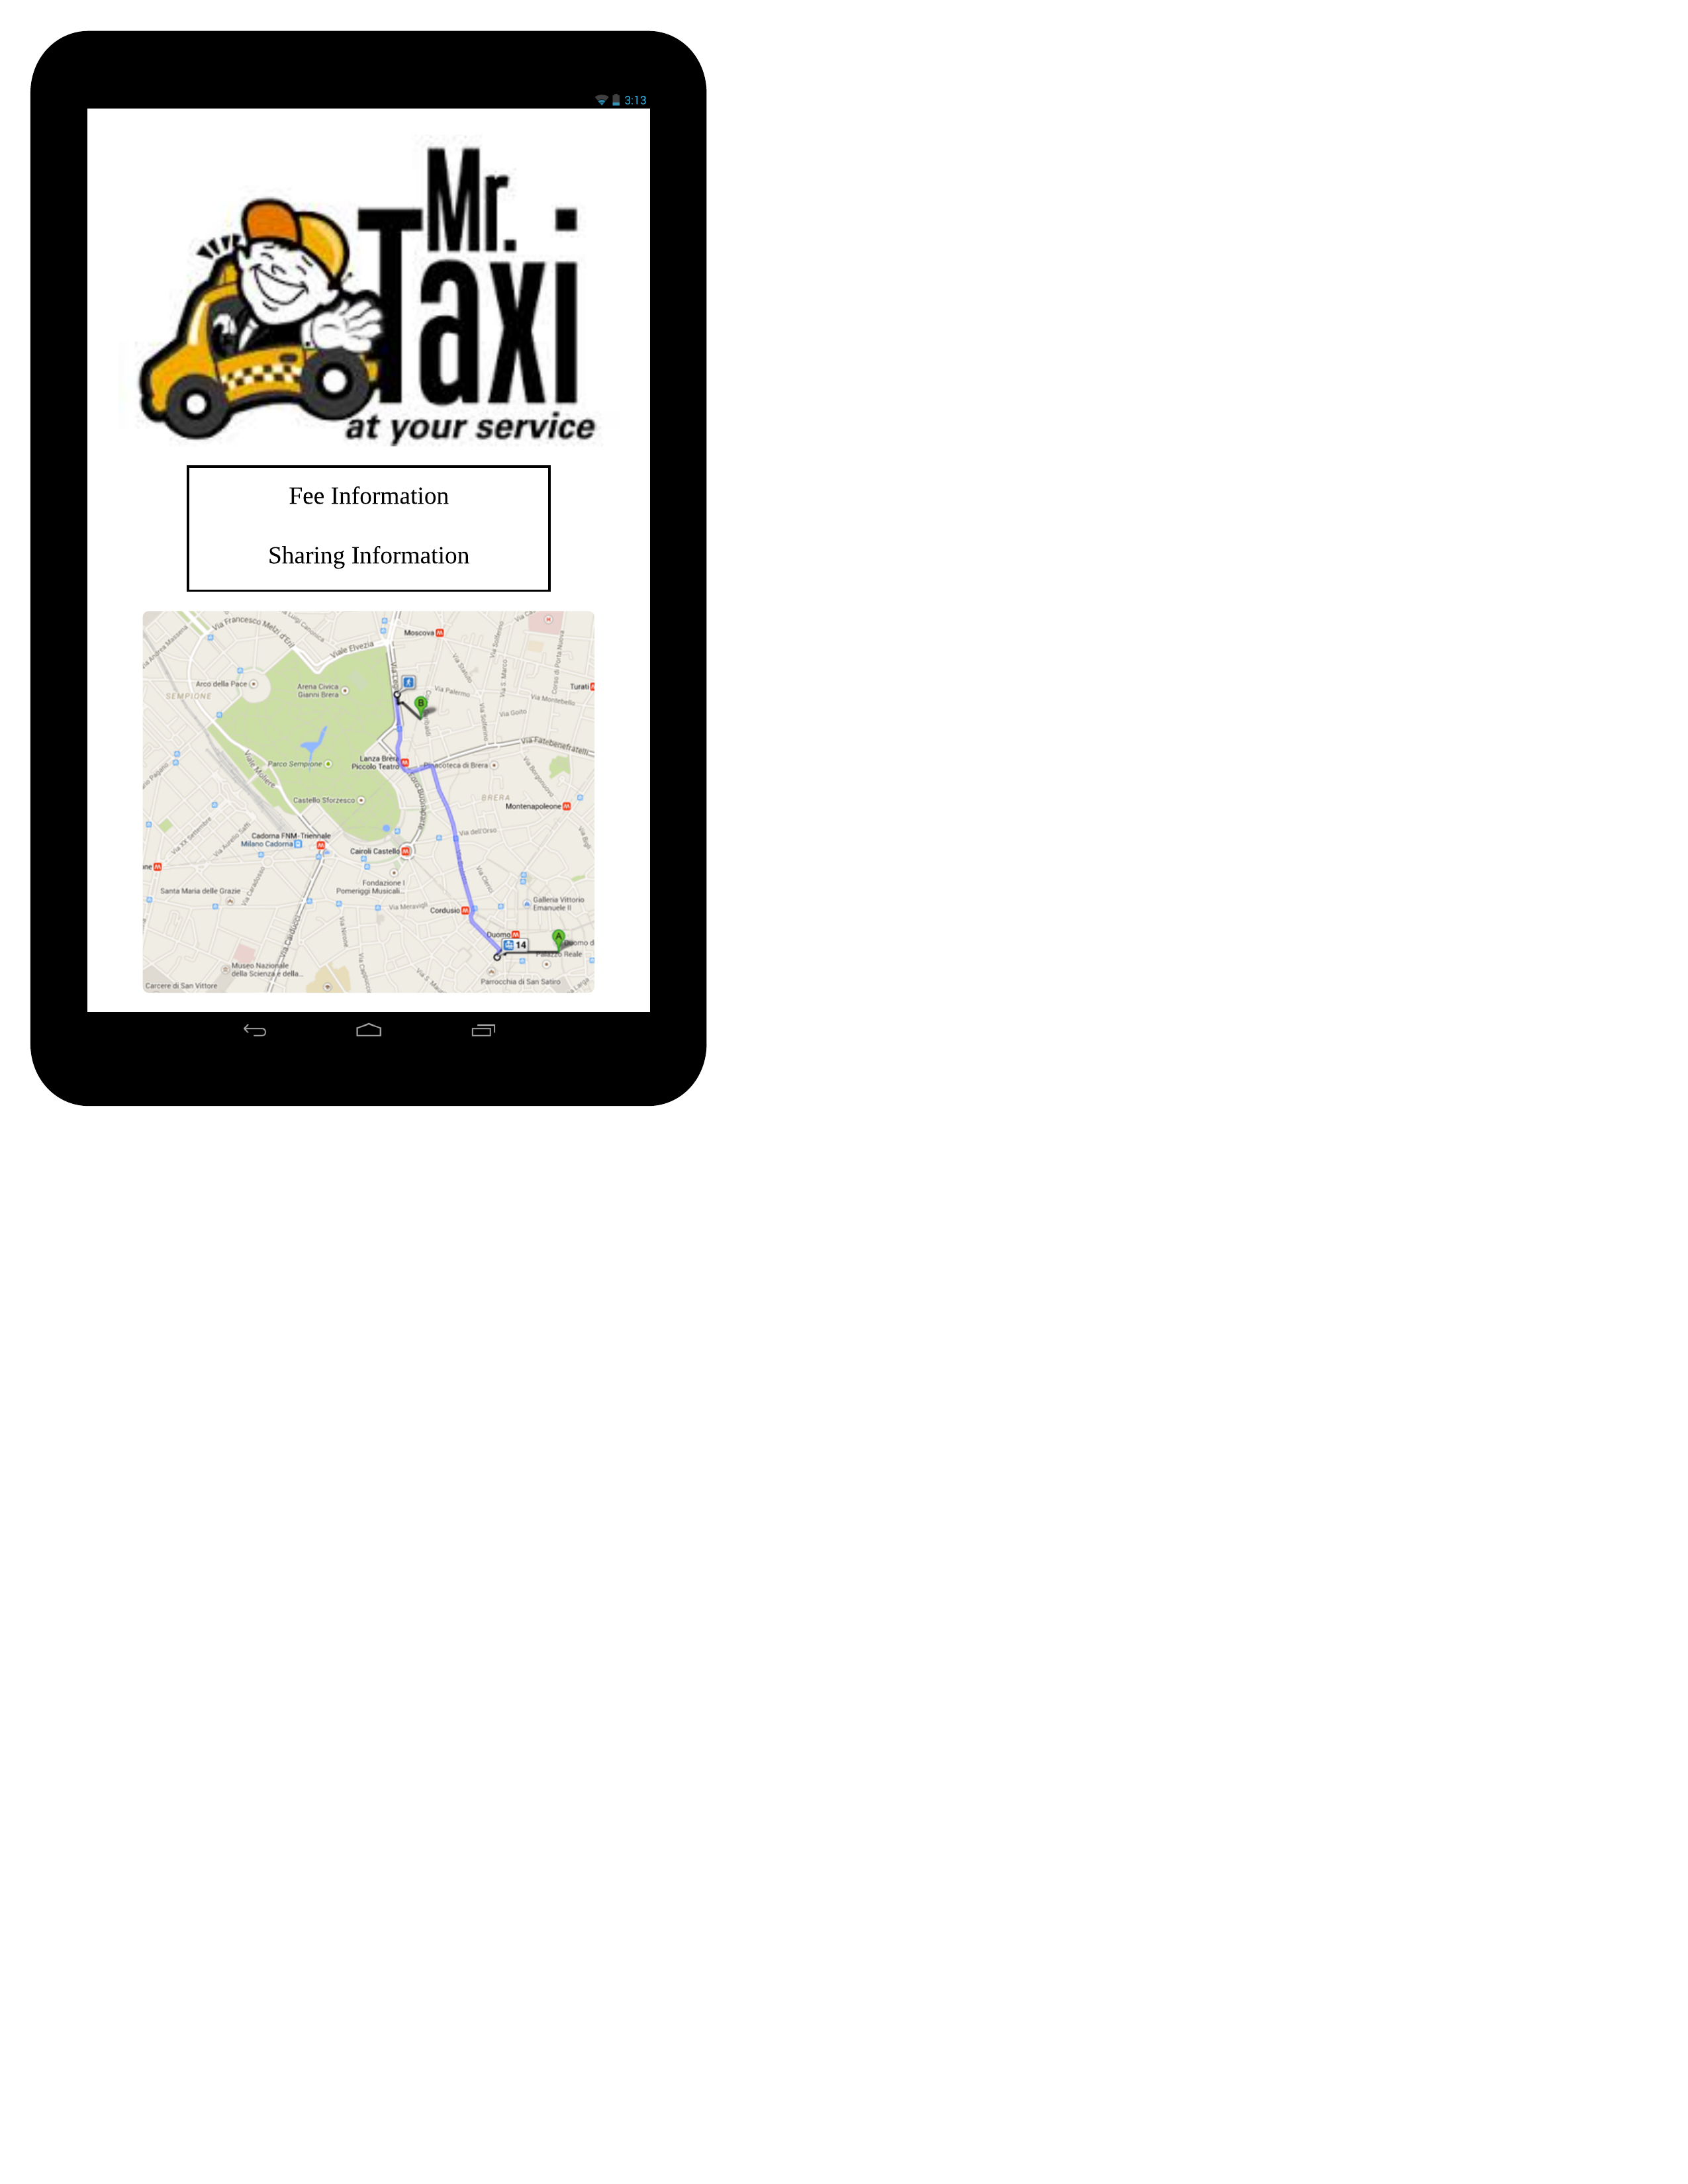
\includegraphics[width=\textwidth]{cpt/img/AccPage}
\caption{Taxi Driver Accepted Call Page mockup}
\label{fig:accpage}
\end{figure}